\subsection{What is needed in an \ab{} workflow system?}

\begin{frame}{What is needed in an \ab{} workflow system?}
    There are at least three components:

    \begin{itemize}
        \item Sciency, technical stuff: calculations, input generation, output analysis...
        \item Dispatcher, job scheduler: interacting with \ab{} software, \texttt{mpi}...
        \item User interface: interacting with users
    \end{itemize}
\end{frame}

\subsection{What is \express{}?}

\begin{frame}{\subsecname}
    \begin{definitionblock}{\express{}}
        A workflow framework consisting of several extensible, lightweight, high-throughput,
        high-level Julia packages that aims to automate \ab{} calculations for the materials
        science community.
    \end{definitionblock}

    We will mention \texttt{Express.jl} later, but beware that it is different from the
    project \express{}. We sometimes say \texttt{Express.jl} and \texttt{Express}
    interchangeably.

    \begin{definitionblock}{\texttt{Express.jl}}
        The core package of the \express{} project, which manages and dispatches the rest
        packages in \express{}.
    \end{definitionblock}
\end{frame}

\begin{frame}[allowframebreaks]{What does \express{} include?}
    \begin{figure}[H]
        \centering
        \makebox[\textwidth][c]{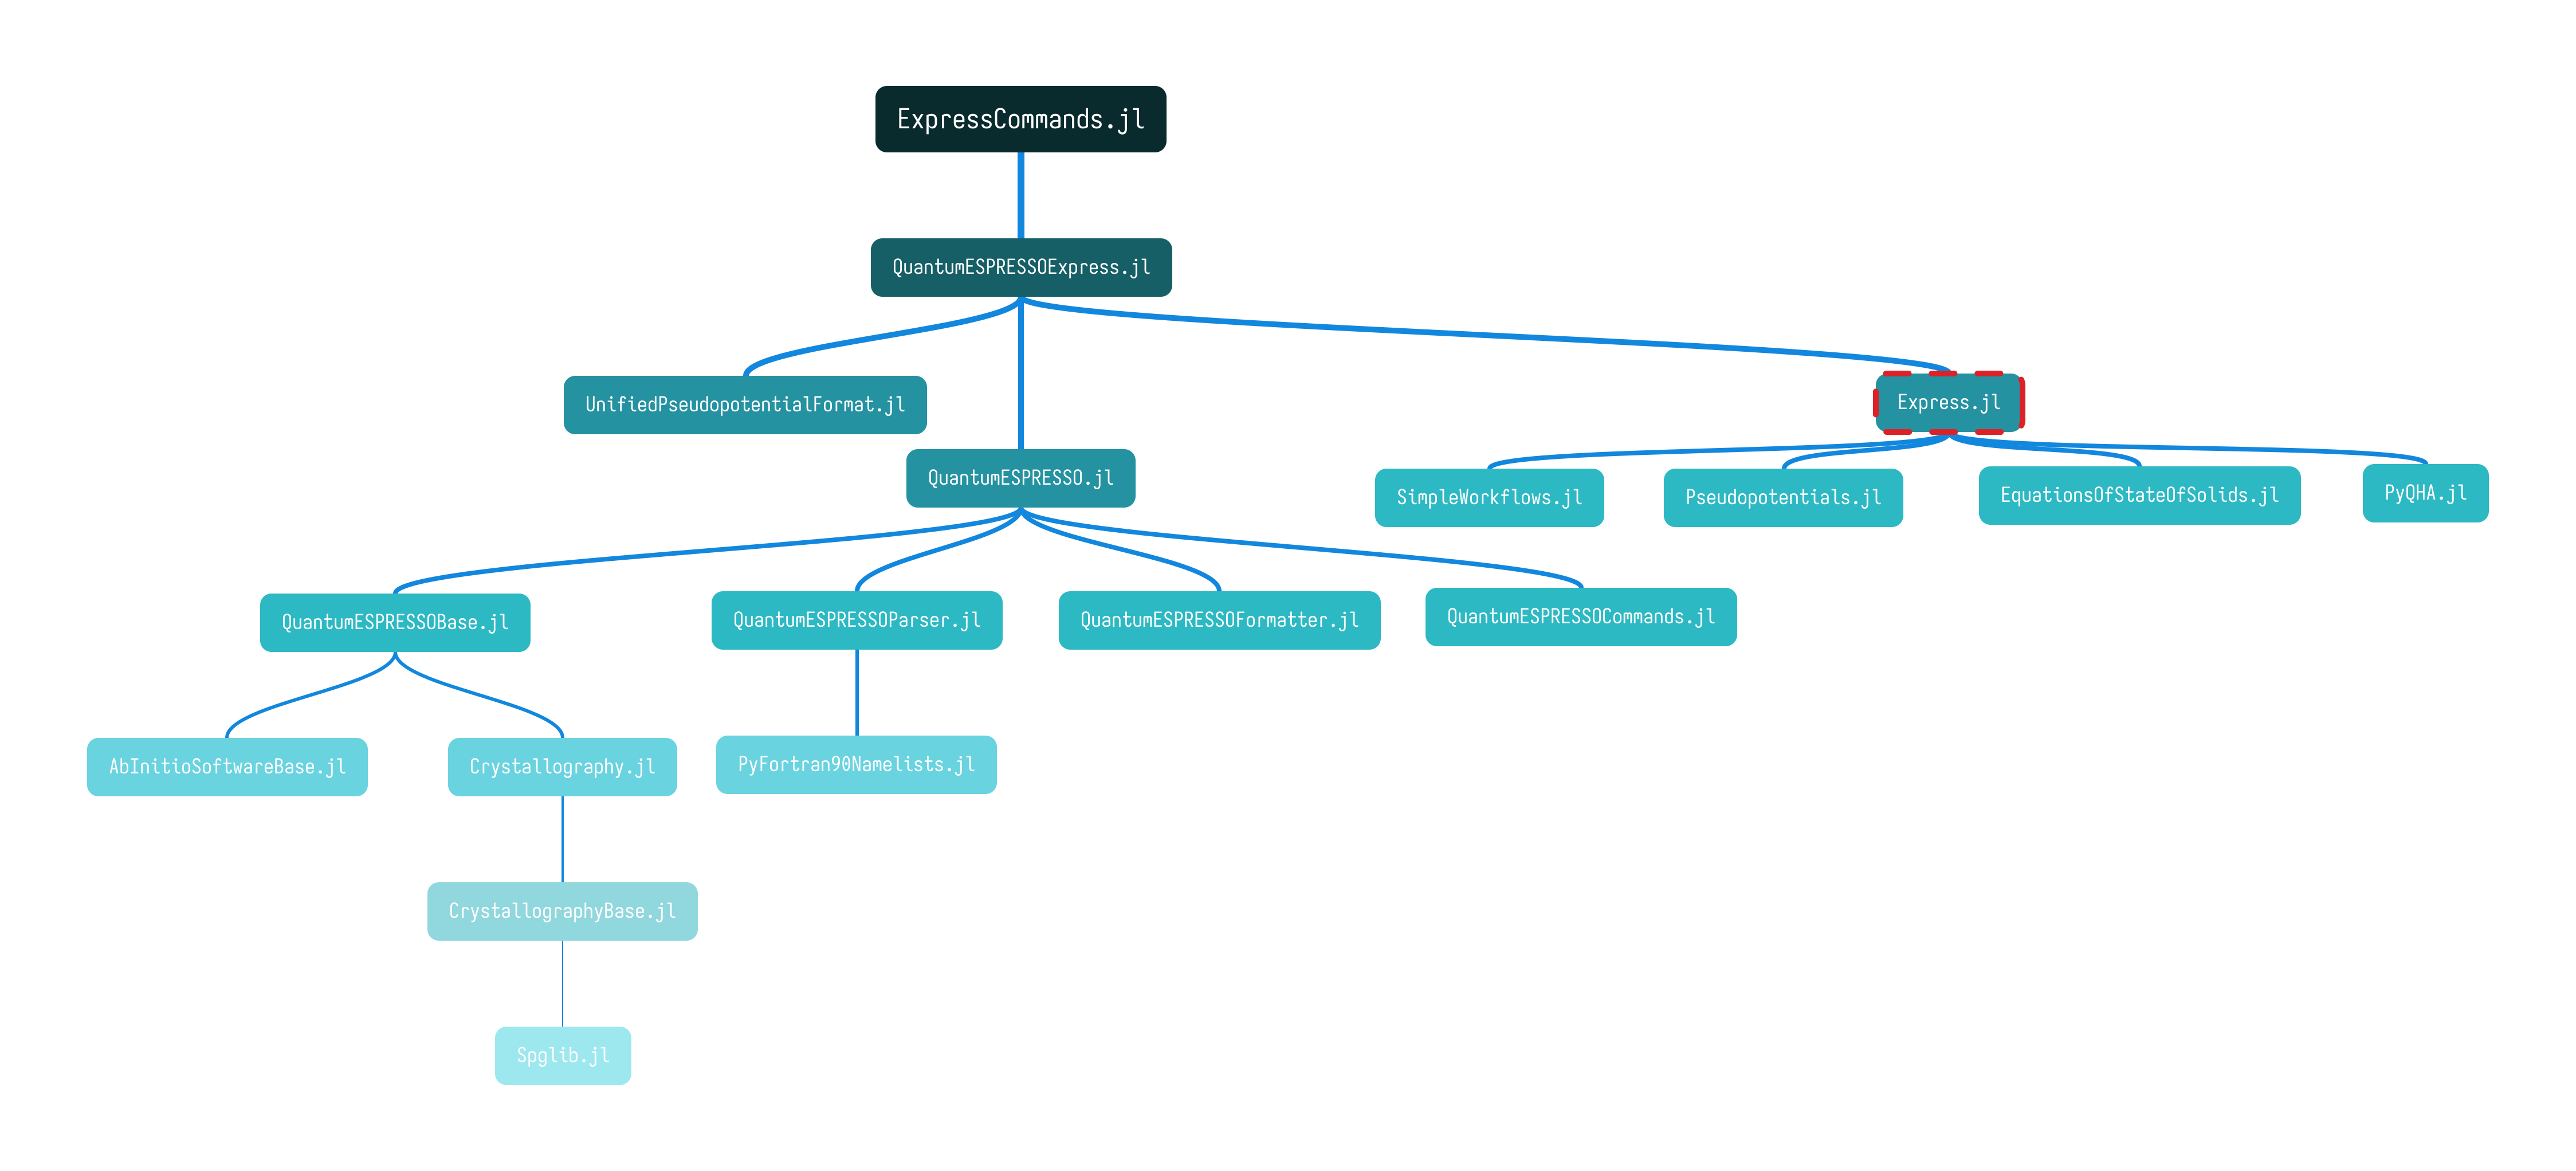
\includegraphics[width=0.9\pagewidth]{components}} % See https://tex.stackexchange.com/a/16584/61591
        \caption{Main components of the \express{} project}
        \label{fig:components}
    \end{figure}

    \framebreak

    \express{} can be separated into two parts: software-neutral and software-specific packages.
    For the first kind, it includes
        {\footnotesize
            \begin{itemize}
                \item \href{https://github.com/MineralsCloud/Express.jl}{\texttt{Express.jl}}
                      provides a high-level interface to all the
                      workflows: file I/O, job scheduling, data analysis, etc.
                      To work with specific software, install the corresponding plugin.
                \item \href{https://github.com/MineralsCloud/ExpressCommands.jl}{\texttt{ExpressCommands.jl}}
                      is a CLI of \texttt{Express.jl}. It installs an executable
                      `\texttt{xps}' which executes code from configuration files.
                \item \href{https://github.com/MineralsCloud/EquationsOfStateOfSolids.jl}{\texttt{EquationsOfStateOfSolids.jl}}
                      fits $E(V)$ data to equations of state.
                \item \href{https://github.com/MineralsCloud/Crystallography.jl}{\texttt{Crystallography.jl}}
                      calculates cell volumes from lattice constants, finds symmetry
                      operations and generates high symmetry points in the Brillouin zone, etc.
                \item \href{https://github.com/MineralsCloud/PyQHA.jl}{\texttt{PyQHA.jl}}
                      is a Julia wrapper of
                      the Python \texttt{qha} package, which can calculate
                      several thermodynamic properties of both single- and multi-configuration
                      crystalline materials in the framework of quasi-harmonic approximation.
                \item \href{https://github.com/MineralsCloud/Pseudopotentials.jl}{\texttt{Pseudopotentials.jl}} presents
                      a database for storing and querying pseudopotentials used in \ab{} calculations.
                \item \href{https://github.com/MineralsCloud/SimpleWorkflows.jl}{\texttt{SimpleWorkflows.jl}}
                      is the skeleton of the workflow system, which
                      defines building blocks, composition rules, and operation order of workflows.
            \end{itemize}
        }

    For the second part, since we currently only support \qe{}, it now includes:
    {\footnotesize
    \begin{itemize}
        \item \href{https://github.com/MineralsCloud/QuantumESPRESSOBase.jl}{\texttt{QuantumESPRESSOBase.jl}}
              declares basic data types and methods
              for manipulating crystal structures, generating input files for \qe{},
              error checking before running, etc.
        \item \href{https://github.com/MineralsCloud/QuantumESPRESSOParser.jl}{\texttt{QuantumESPRESSOParser.jl}}
              parses the I/O files of \qe{} to extract and analyze data.
        \item \href{https://github.com/MineralsCloud/QuantumESPRESSOFormatter.jl}{\texttt{QuantumESPRESSOFormatter.jl}}
              formats the input files of \qe{}.
        \item \href{https://github.com/MineralsCloud/QuantumESPRESSOCommands.jl}{\texttt{QuantumESPRESSOCommands.jl}}
              is a CLI that exports the commands of \qe{} in a configurable way.
        \item \href{https://github.com/MineralsCloud/QuantumESPRESSO.jl}{\texttt{QuantumESPRESSO.jl}}
              is simply a wrapper of the types, methods, and commands defined in
              the four packages mentioned above.
        \item \href{https://github.com/MineralsCloud/QuantumESPRESSOExpress.jl}{\texttt{QuantumESPRESSOExpress.jl}}
              is a plugin of \texttt{Express.jl} for handling \ab{} software such as \qe{}.
    \end{itemize}
    }
\end{frame}
